Our submarine design consists of 4 overall design systems. The control system, the movement system, the debris collection system and the visual system. The overall system works together delivering data between these various sub systems in order to insure that the pilot of the submarine can accurately execute actions related to operating the submarine.

\begin{figure}[h!]
	\centering
 	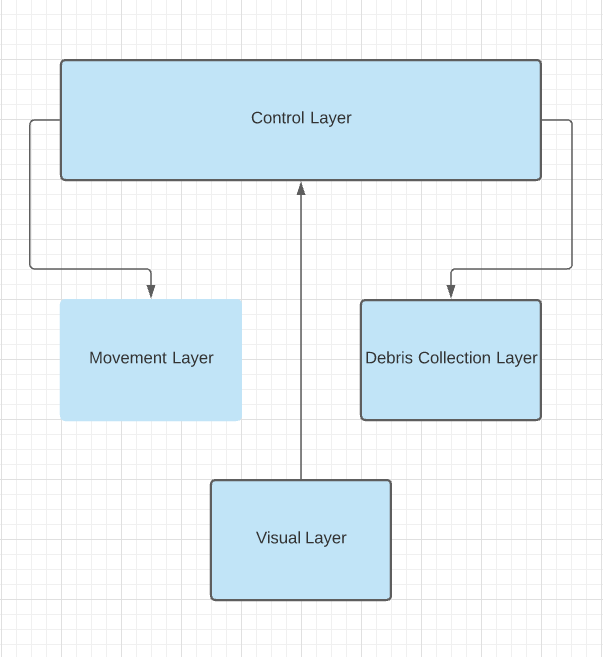
\includegraphics[width=0.60\textwidth]{images/layers}
 \caption{A simple architectural layer diagram}
\end{figure}

\subsection{Control Layer Description}
The control layer involves using the library ArduPilot to call a control system that will operate the underwater vehicle on 6 degrees of freedom. As such the vehicle will need the capability of turning on all axis as well as horizontal spins. It will send its commend through the tether connected to the vehicle and the motor operation will be updated according to the library specifications. The ArduSub sublibrary of the ArduPilot series of libraries has a specification with motor placement that must be followed in order to achieve full functionality from the library.

The control layer also receives input data through the tether from the visual system. That input data is displayed for the pilot onto a monitor system which contains an overlay with some targeting assistance graphics built on top of the display.

All of this data is manipulated through the tether which connects our generic RV controller with micro-controllers installed directly on the vehicle. The vehicle itself will contain between 2-4 micro-controllers that will be responsible for turning on and off the electrical signals.

\subsection{Movement Layer Description}
The movement layer currently consists of a set of 6 thrusters. The thrusters must be placed at predefined specified locations to conform to ArduPilot library's prebuilt specifications. In order to obtain 8 degrees of freedom we will need 2 rear thrusters, and then 4 thrusters placed at various points in a circular fashion all differing by 45 degrees from eachother. The thrusters are turned off and on via electrical signals from micro controllers installed on the vehicle in the control layer. The directional capability of the movement system is all handled automatically by ArduPilot, our system will only implement the thrusters in the specifications according to the ArduPilot library.

\subsection{Debris Collection Layer Description}
The debris collection layer consists of a mechanical arm to collect sunken debris, and a net pulley system to collect floating debris. The net pulley system will collect the floating debris and deposit the debris into a catapult system which will then launch the debris into the collection area. The mechanical arm system will receive signals to clasp the sunken debris from the control system and then release it via the same control system.

\subsection{Visual Layer Description}
The visual layer is the one layer that is meant to deliver information back to the control layer. The information is collected through a waterproof camera on the front of the submarine and then transmitted through the tether to be displayed on the monitor of the control system.  